%%This is a very basic article template.
%%There is just one section and two subsections.
\documentclass[parskip=full]{scrartcl}
\usepackage[table]{xcolor}

\usepackage{amsmath}
\usepackage{amsfonts}
\usepackage{mathtools}
\usepackage{studarbeit}
\usepackage{graphicx}
\usepackage{wrapfig}
\usepackage{lscape}
\usepackage{rotating}
\usepackage{epstopdf}
\usepackage{pdfpages}
\usepackage{caption, booktabs}
\usepackage{tabularx}
\usepackage{multirow}
\usepackage{here}
\usepackage[most]{tcolorbox}
\usepackage[binary-units=true]{siunitx}
 \usepackage[autostyle=true,german=quotes]{csquotes}
 \usepackage{longtable, booktabs}
 \newcommand{\swtLabel}[1]{\textbf{/#1\arabic*0/}}
 \definecolor{testgrauRGB}{rgb}{0.9,0.9,0.9}
 \definecolor{myGreen}{cmyk}{1,0.0,1,0}
 \newlist{itemMinus}{itemize}{1 }
 \setlist[itemMinus]{label=--, noitemsep,
 before=\color{red}\normalfont\ttfamily}
  \newlist{itemPlus}{itemize}{1 }
  
 \setlist[itemPlus]{label=+,noitemsep,before=\color{myGreen}\normalfont\ttfamily}
  \newlist{itemPackage}{itemize}{1 }
 \setlist[itemPackage]{label=*,noitemsep, before=\ttfamily\itshape}
  \newlist{itemClass}{itemize}{1 }
 \setlist[itemClass]{label=~,noitemsep,before=\normalfont\ttfamily}
 \newlist{itemClassSub}{itemize}{1 }
 \setlist[itemClassSub]{label=~,noitemsep,before=\normalfont}
\newlist{itemChange}{itemize}{1 }
 \setlist[itemChange]{label=>,noitemsep,before=\color{blue}\normalfont\ttfamily}
 \setlist[itemize]{label=~,before=\normalfont}
  \newcommand{\changeDescription}[1]{{\newline\color{black}\normalfont #1}}
  \newcommand{\code}[1]{{\ttfamily #1}}
 \begin{document}

\title{Elipse -- Einteilungs Interface für das PSE}
\author{D. Biester, E. Dohse, P. Faller, P. Loth, L. Seufert, S. Kopmann}
\thesistype{Implementierungsdokument}
\zweitgutachter{}
\betreuer{Dipl.-Inform.~Andreas~Zwinkau, M.Sc.~Andreas~Fried}
\coverimage{ElipseLogo.png}
\mytitlepage
{\setlength{\textheight}{297mm}
\tableofcontents

\setlength{\textheight}{297mm}}
\pagebreak

\section{Einleitung}

Nachdem im Pflichtenheft beschrieben wurde, was das Produkt leisten soll und
das Entwurfsdokument beantwortete, wie das Produkt strukturiert sein soll, 
beschreibt dieses Dokument nun die Implementierung, also die Umsetzung der beiden vorherigen Dokumente.

\section{Implementierungsplan}
Zu beginn der Implementierungsphase wurde ein Plan erstellt, der unser
vorgesehenes Vorgehen beschreibt.
%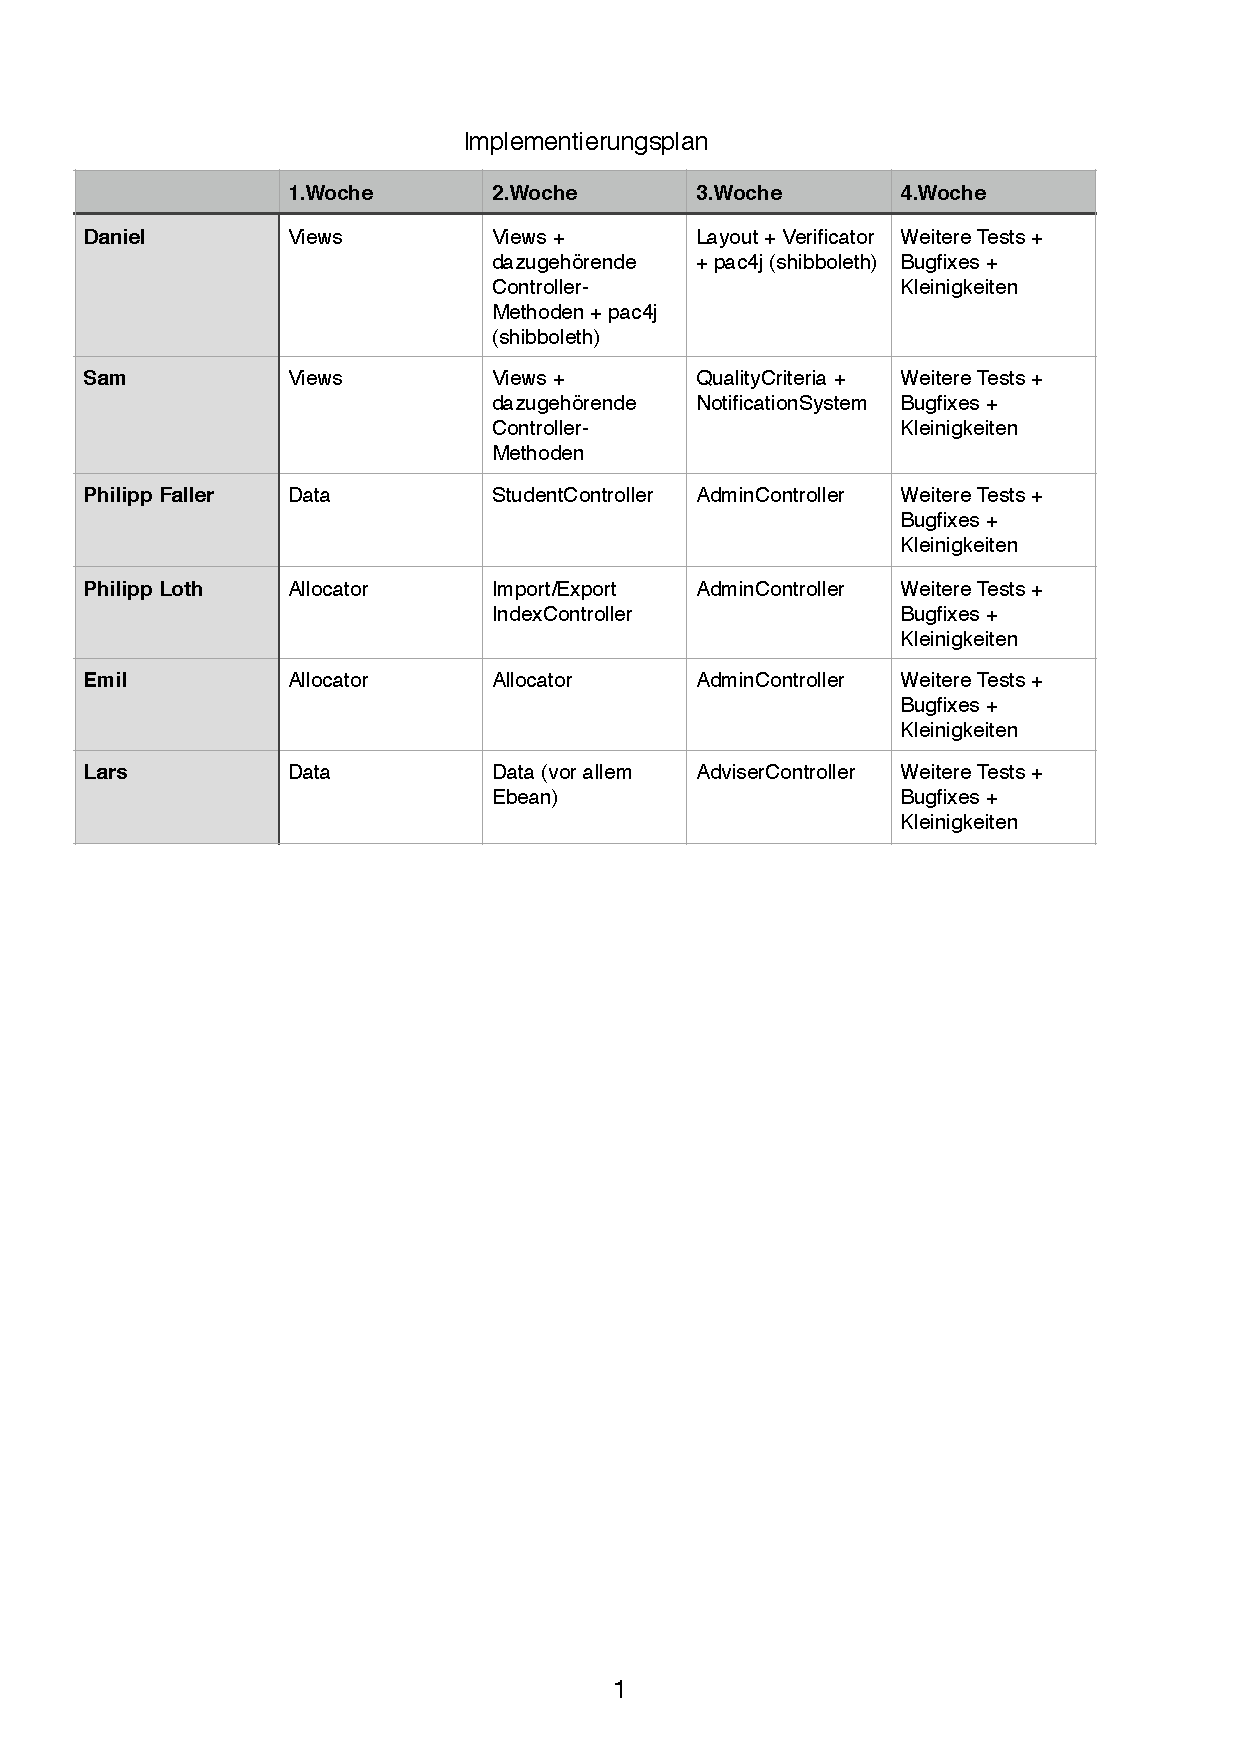
\includepdf[pages={1}]{Implementierungsplan.pdf}

\begin{table}[H]
\begin{tabularx}{\textwidth}{|l|l|X|X|X|}
\hline
 	& 1. Woche			& 2. Woche		& 3. Woche & 4. Woche\\
\hline 
Daniel	& Views			& Views + dazu-gehörende Controller-Methoden + pac4j 
(shibboleth) & Layout + Verificator
+ pac4j (shibboleth)& Weitere Tests +
Bugfixes +
Kleinigkeiten\\
\hline
Sam & Views&Views +
dazu-gehörende
Controller-
Methoden & QualityCriteria +
NotificationSystem & Weitere Tests +
Bugfixes +
Kleinigkeiten\\
\hline
Philipp Faller&Data&Import/Export
IndexController&AdminController&Weitere Tests +
Bugfixes +
Kleinigkeiten\\
\hline
Philipp Loth&Allocator&Import/Export
IndexController&AdminController&Weitere Tests +
Bugfixes +
Kleinigkeiten\\
\hline
Emil&Allocator&Allocator&AdminController&Weitere Tests +
Bugfixes +
Kleinigkeiten\\
\hline
Lars&Data&Data (vor allem
Ebean)&AdviserController&Weitere Tests +
Bugfixes +
Kleinigkeiten\\
\hline
\end{tabularx}
\caption{Implementierungsplan}
\end{table}
% Hierbei war der für uns \enquote{kritische Pfad} %TODO Was ist unser Criticall
% % Path 
% das das Datenmodell gefolgt von paralell implementierbaren Controllern die nur
% auf das Datenmodell zugreiffen und der Allocation. 
Der Critical"=Path unseres Entwurfs startet, bedingt durch das Model"=View"=Controller"=Design, ganz klar beim Package \code{data} und verläuft über \code{allocator}, gefolgt von \code{controller} zu  \code{views}.
Da wir jedoch vermuteten, dass der meiste Code bei den Controllern anfallen würde, sowie dass das Einarbeiten \enquote{Play} mit seiner \enquote{Twirl"=Template"=Engine} lange dauern würde, haben wir beschlossen, schon von Anfang an diesen beiden Baustellen zu arbeiten. 
Außerdem hat sich jeder von uns bereits in der Entwurfsphase auf ein Gebiet spezialisiert und es bot sich somit an, jedem auf seinem \enquote{Fachgebiet} auch die Implementierung zu übertragen.
Diese Prognose war nur teilweise richtig.
Zwar hat tatsächlich das Package \code{controller} mit Abstand die meisten Zeilen Quellcode, jedoch haben wir den Aufwand für die Einrichtung unseres ORMs \enquote{Ebean} weit unterschätzt. 
Durch die häufig kryptischen Fehlermeldungen und spärliche (bis hin zu schlicht falsche) Dokumentation zog sich das Implementieren des Datenmodells bis an den Anfang der dritten Woche. 
Da jedoch parallel dazu ständig an den anderen Paketen gearbeitet wurde, war als die Datenbank endlich funktionierte schon eine große Menge Code vorhanden, weswegen vor allem zum Schluss hin sehr schnell viel Funktionalität hinzugefügt werden konnte.
Die Implementierung des Paket \code{allocation} verlief ausgesprochen gut.

Insgesamt haben wir uns also bis auf die Datenbank an den Implementierungsplan halten können. Dort mussten wir jedoch starke Verzögerungen in Kauf nehmen.

%TODO zweites Diagramm wie haben wir wirklich implementeirt

%dann fairness bzw hierzu nur einen satz aber allgemeine statistiken 


\begin{table}[H]
\begin{tabularx}{\textwidth}{|l|l|X|X|X|}
\hline
 	& 1. Woche			& 2. Woche		& 3. Woche & 4. Woche\\
\hline 
Daniel	& Views			& Views + dazu-gehörende Controller-Methode & Layout + Verificator
+ pac4j&Deadlines + Bugfixes +
Kleinigkeiten \\
\hline
Sam & Views&Views& QualityCriteria +
NotificationSystem & Weitere Tests +
Bugfixes +
Kleinigkeiten\\
\hline
Philipp Faller&Data&Data&Bugfixes&Bugfixes +  Email\\
\hline
Philipp Loth&Allocator&Import/Export
&Import/Export + Kleinigkeiten &Weitere Tests +
Bugfixes +
Form Validation\\
\hline
Emil&Allocator&Controller&Controller&Form Validation +
Bugfixes +
Kleinigkeiten\\
\hline
Lars&Data&Data (vor allem
Ebean)&Controller + Daten &
Controller-Bugfixes +
Kleinigkeiten\\
\hline
\end{tabularx}
\caption{Wirkliche Implementierung}
\end{table}
\section{Änderungen zum Entwurfsdokument}
Zur Sicherung bessere Code-Qualität (z.B. dem Vermeiden von Code-Copy-Pasting)
und maßgeblich durch die oben beschriebenen Probleme mit verschiedenen
verwendeten Bibliotheken  wurden Änderungen im Vergleich zum  Entwurfsdokument
vorgenommen. 
Dabei wurden die Getter, Setter und Konstruktoren der Vollständigkeit halber
eingefügt und werden hier nicht weiter kommentiert.
%TODO Auch atribute nicht kommentieren?
\begin{itemPackage}
\item allocation
\begin{itemClass}
\item AbstractAllocator
\begin{itemClassSub}
\item Methoden
\begin{itemPlus}
\item cancel() \changeDescription{Um eine Einteilungsberechnung durchzuführen
wird diese Methode benötigt.}
\item init(Configuration)\changeDescription{Um Race-Conditions zu vermeiden
wurde diese Methode eingefügt. Mit ihr können \code{init()} und \code{cancel()}
synchronised werden ohne calculate zu blockieren.}
\end{itemPlus}
\begin{itemChange}
\item calculate() \changeDescription{Die Konfiguration wird bereits bei
\code{init()} übergeben.}
\end{itemChange}
\end{itemClassSub}
\item AllocationQueue
\begin{itemClassSub}
\item Methoden
\begin{itemPlus}
\item clear() \changeDescription{Leert die Queue, wird in Unit-Tests verwendet.}
\item getAllocator() : AbstractAllocator
\end{itemPlus}
\begin{itemChange}
\item cancelAllocation(String)
\end{itemChange}
\item Attribute
\begin{itemPlus}
\item allocator : AbstractAllocator \changeDescription{Zur Realisierung des
Strategiemusters.}
\end{itemPlus}
\end{itemClassSub}
\item Configuration
\begin{itemClassSub}
\item Methoden
\begin{itemPlus}
\item getTeams() : List<Team> 
\end{itemPlus}
\begin{itemMinus}
\item getProjects() : List<Project> 
\end{itemMinus}
\item Konstruktoren
\begin{itemPlus}
\item Configuration(String, List<Student>, List<LearningGroup>, List<Project>,
List<AllocationParameter>)
\end{itemPlus}
\item Atribute
\begin{itemPlus}
\item teams : List<Team> \changeDescription{Die Teams werden bei der
Einteilungsberechnung benötigt und aus den im Konstruktor übergebenen
Projekten berechnet.}
\end{itemPlus}
\begin{itemMinus}
\item projects : List<Project> \changeDescription{Werden implizit durch die
Teams gespeichert.}
\end{itemMinus}
\end{itemClassSub}
\item Criterion
\begin{itemClassSub}
\item Methoden
\begin{itemPlus}
\item getDisplayName(String) : String \changeDescription{Zur
internationalisierung Benutzeroberfläche in Abgrenzung zu \code{getName()}.}
\end{itemPlus}
\end{itemClassSub}
\item GurobiAllocator
\begin{itemClassSub}
\item Parameter
\begin{itemPlus}
\item currentConfiguration : Configuration \changeDescription{Wird zum Abbruch
der Einteilungsberechnung benötigt.}
\end{itemPlus}
\end{itemClassSub}
\item GurobiCriterion
\begin{itemClassSub}
\item Methoden
\begin{itemChange}
\item useCriteria(Configuration, GurobiAllocator, double)
\changeDescription{\code{GurobiAllocator} wird von Kriterien benötigt.}
\end{itemChange}
\end{itemClassSub}
\end{itemClass}
\item controller
\begin{itemClass}
\item AdminEditAllocationController
\begin{itemClassSub}
\item Methoden
\begin{itemPlus}
\item editAllocation() : Result \changeDescription{Diese Methode gibt das
\code{DynamicForm} an die Methoden \code{moveStudents(DynamicForm, List<Integer>)} und
\code{swapStudents(DynamicForm, List<Integer>)} weiter, wenn der Administrator
eine Allocation bearbeitet. }
\end{itemPlus}
\begin{itemChange}
\item moveStudents(DynamicForm, List<Integer>) : Result\changeDescription{Methode zur Weitergabe des \code{DynamicForm} an den
\code{Command}.}
\item swapStudents(DynamicForm, List<Integer>) : Result
\changeDescription{Methode zur Weitergabe des \code{DynamicForm} an den
\code{Command}.}
\end{itemChange}
\end{itemClassSub}
\item AdminImportExport
\item \begin{itemClassSub}
\item Methoden
\begin{itemPlus}
\item importGeneral() : Result \changeDescription{Leitet das Drücken des
Import-Knopfs an die Import-Methoden weiter.}
\item exportGrades() : Result \changeDescription{Da das CMS-Format unbekannt
ist, ein allgemeiner Notenexport.}
\end{itemPlus}
\end{itemClassSub}
\item AdminPageController
\item \begin{itemClassSub}
\item Methoden
\begin{itemPlus}
\item accountPage() : Result \changeDescription{Zusatzfeature, damit der
Administrator sein Passwort ändern kann.}
\item notAllowedInCurrentState(String) : Result \changeDescription{Methode die
zur Umsetzung von Deadlines gebraucht wird.}
\end{itemPlus}
\begin{itemChange}
\item projectEditPage(int) : Result \changeDescription{\code{int} für das
Weiterleiten an ein Projekt mit der Id \code{int}. }
\end{itemChange}
\end{itemClassSub}
\item AdminPropertiesController
\item \begin{itemClassSub}
\item Methoden
\begin{itemPlus}
\item changeSPO() : Result \changeDescription{Ersatz und Erweiterung für
\code{removeAchievement()}. }
\item editSMTPOptions() : Result \changeDescription{Wird für die Konfiguration
des E-Mail-Servers (SMTP) verwendet.}
\end{itemPlus}
\begin{itemMinus}
\item removeAchievement() : Result \changeDescription{Wurde durch
\code{changeSPO()} ersetzt.}
\end{itemMinus}
\end{itemClassSub}
\item AdviserPageController
\item \begin{itemClassSub}
\item Methoden
\begin{itemPlus}
\item notAllowedInCurrentState(String) : Result \changeDescription{Methode die
zur Umsetzung von Deadlines gebraucht wird}
\end{itemPlus}
\end{itemClassSub}
\item GeneralAdminController
\item \begin{itemClassSub}
\item Methoden
\begin{itemPlus}
\item removeAllocationFromQueue() : Result \changeDescription{Wird zum Abbruch
der Einteilungsberechnung benötigt.}
\item editAccount() : Result \changeDescription{Zusatzfeature, wird zum
Bearbeiten des Adminaccounts verwendet.}
\end{itemPlus}
\end{itemClassSub}
\item IndexPageController
\item \begin{itemClassSub}
\item Methoden
\begin{itemPlus}
\item notAllowedInCurrentState(String) : Result \changeDescription{Methode die
zur Umsetzung von Deadlines gebraucht wird.}
\item passwordResetForm() : Result \changeDescription{View für Studierende, die
ihr Passwort vergessen haben und es zurücksetzen müssen.}
\item resetPassord(String) : Result \changeDescription{Methode zum
Passwort-Reset von Studenten}
\end{itemPlus}
\begin{itemMinus}
\item login() : Result \changeDescription{Wird von \code{pac4j} übernommen.}
\item passwordReset() : Result \changeDescription{Wurde durch
\code{resetPassord(String)} ersetzt}
\end{itemMinus}
\end{itemClassSub}
\item MoveStudentCommand
\begin{itemClassSub}
\item Konstruktoren
\begin{itemPlus}
\item MoveStudentCommand(Allocation, List<Student>, Team)
\end{itemPlus}
\item Attribute
\begin{itemPlus}
\item oldTeams : Map<Student, Team> \changeDescription{Beim verschieben von 2
verschiedenen Studenten aus 2 verschiedenen Teams muss gespeichert werden, in
welchem Team die Beiden ursprünglich waren. Nur dann kann man die Änderung
rückgängig machen.}
\item students : List<Student> \changeDescription{Nun kann mehr als ein Student
auf einmal verschoben werden.}
\end{itemPlus}
\begin{itemMinus}
\item oldTeam : Team \changeDescription{Wurde durch \code{oldTeams :
Map<Student, Team>} ersetzt}
\item student : Student \changeDescription{Wurde durch \code{students :
List<Student>} ersetzt }
\end{itemMinus}
\end{itemClassSub}
\item StudentPageController
\item 
\begin{itemClassSub}
\item Methoden
\begin{itemPlus}
\item changeData() : Result \changeDescription{Zur Änderung der Daten eines
Studenten, z.B. wenn er bei seiner ersten Anmeldung nicht zugeteilt wurde und
nun in einem höheren Semester ist}
\item changeFormPage() : Result \changeDescription{Der View für
\code{changeData()} }
\item notAllowedInCurrentState(String) : Result \changeDescription{Methode die
zur Umsetzung von Deadlines gebraucht wird.}
\item sendNewVerificationLink() : Result \changeDescription{Wenn die E-Mail bei
der Verifikation der E-Mail-Adresse nicht ankommt kann hier eine neue E-Mail
angefordert werden }
\item setLearningGroup() : Result \changeDescription{Leitet an die bereits
existierenden Methoden \code{joinLearningGroup()} und
\code{createLearningGroup} weiter.}
\end{itemPlus}
\end{itemClassSub}
\item SwapStudent
\begin{itemClassSub}
\item Konstruktoren
\begin{itemPlus}
\item SwapStudentCommand(Allocation, Student, Student) \changeDescription{}
\end{itemPlus}
\end{itemClassSub}
\end{itemClass}
\item data
\begin{itemClass}
\item Administrator
\begin{itemize}
  \item Klasse hinzugefügt, da er nun auch als \code{User} in der Datenbank
  liegt.
\end{itemize}
\item ElipseModel
\begin{itemize}
  \item Klasse als Oberklasse für alle Datenklassen hinzugefügt, um
  \code{equals}-Methoden und ähnliches einheitlich zu behandeln.
\end{itemize}
\item Grade
\begin{itemize}
  \item Enum hinzugefügt, um Noten darzustellen
\end{itemize}
\item Transaction
\begin{itemize}
  \item Interface hinzugefügt, um das Speichern beim Durchführen von Änderungen
  an Datenobjekten zu Automatisieren.
\end{itemize}
\item Achievement
\begin{itemClassSub}
\item Methoden
\begin{itemPlus}
\item compareTo(Achievement) : int \changeDescription{Um \code{Achievments} zur
Anzeige zu Sortieren }
\end{itemPlus}
\item Konstruktoren
\begin{itemPlus}
\item Achievement(String)
\end{itemPlus}
\end{itemClassSub}
\item Adviser
\item \begin{itemClassSub}
\item Methoden
\begin{itemPlus}
\item getProjects(): List<Project>
\end{itemPlus}
\begin{itemMinus}
\item addProject(Project) \changeDescription{\code{Projects} werden nicht mehr
bei \code{Advisers} gespeichert}
\item removeProject(Project)\changeDescription{\code{Projects} werden nicht mehr
bei \code{Advisers} gespeichert}
\end{itemMinus}
\item Konstruktoren
\begin{itemPlus}
\item Adviser(String, String, String, String)
\end{itemPlus}
\end{itemClassSub}
\item Allocation
\item \begin{itemClassSub}
\item Methoden
\begin{itemPlus}
\item getSemester() : Semester
\item setSemester(Semester)
\item getTeam(Student) : Team
\item setStudentsTeam(Student, Team)
\item getTeamsByAdviser(Adviser) : List<Team>
\item getTeamsByProject(Project) : List<Project>
\item getNotAllocatedStudents() : List<Student>
\end{itemPlus}
\begin{itemMinus}
\item clone() : Allocation \changeDescription{Wird von Konstruktor
\code{Allocation(Allocation)} übernommen}
\end{itemMinus}
\item Konstruktoren
\begin{itemPlus}
\item Allocation(List<Team>, String, List<AllocationParameter>)
\item Allocation(Allocation)
\end{itemPlus}
\item Attribute
\begin{itemPlus}
\item semester : Semester \changeDescription{Wird von Ebean benötigt}
\end{itemPlus}
\end{itemClassSub}
\item AllocationParameter
\begin{itemClassSub}
\item Konstruktoren
\begin{itemPlus}
\item AllocationParameter(String, int)
\end{itemPlus}
\end{itemClassSub}
\item GeneralData
\begin{itemClassSub}
\item Methoden
\begin{itemPlus}
\item loadInstance() : GeneralData \changeDescription{Läd alle Daten aus der
Datenbank}
\end{itemPlus}
\begin{itemMinus}
\item getAdminName() : String
\item setAdminName(String)
\item getAdminPassword() : String
\item setAdminPassword(String)
\end{itemMinus}
\item Attribute 
\begin{itemMinus}
\item adminName : String \changeDescription{Wird nun in der Klasse
\code{Administrator} gekapselt}
\item adminPassword : String \changeDescription{Wird nun in der Klasse
\code{Administrator} gekapselt}
\end{itemMinus}
\end{itemClassSub}
\item LearningGroup
\begin{itemClassSub}
\item Methoden
\begin{itemPlus}
\item getSemester() : Semester
\item setSemester(Semester)
\item addMember(Student) \changeDescription{\code{Students} werden nun bei
\code{LearningGroups} gespeichert nicht andersherum}
\item removeMember(Student)\changeDescription{\code{Students} werden nun bei
\code{LearningGroups} gespeichert nicht andersherum}
\end{itemPlus}
\item Konstruktoren
\begin{itemPlus}
\item LearningGroup(String, String)
\item LearningGroup(String, String, Student, boolean)
\end{itemPlus}
\item Attribute 
\begin{itemPlus}
\item semester : Semester \changeDescription{Durch Ebean bedingtes Attribut}
\end{itemPlus}
\end{itemClassSub}
\item Project
\begin{itemClassSub}
\item Methoden
\begin{itemPlus}
\item setSemester(Semester)
\item getSemester() : Semester
\item addAdviser(Adviser)
\item removeAdviser(Adviser)
\end{itemPlus}
\begin{itemMinus}
\item getRating(Student) : int
\item getProject(String, Semester) : Project
\end{itemMinus}
\item Konstruktoren
\begin{itemPlus}
\item Project(String, String, String, String)
\end{itemPlus}
\item Attribute 
\begin{itemPlus}
\item semester : Semester \changeDescription{Durch Ebean bedingtes Attribut}
\end{itemPlus}
\end{itemClassSub}
\item Rating
\begin{itemClassSub}
\item Methoden
\begin{itemPlus}
\item getLearningGroup() : LearningGroup
\item setLearningGroup(LearningGroup)
\end{itemPlus}
\item Konstruktoren
\begin{itemPlus}
\item Rating(int, Project)
\end{itemPlus}
\item Attribute 
\begin{itemPlus}
\item learningGroup : LearningGroup \changeDescription{Durch Ebean bedingtes
Attribut}
\end{itemPlus}
\end{itemClassSub}
\item Semester
\begin{itemClassSub}
\item Methoden
\begin{itemPlus}
\item getMaxGroupSize() : int
\item setMaxGroupSize(int)
\item isWintersemester() : boolean
\item setWintersemester(boolean)
\item addAllocation(Allocation)
\item removeAllocation(Allocation)
\item addProject(Project)
\item removeProject(Project)
\item addStudent(Student)
\item removeStudent(Student)
\item addLearningGroup(LearningGroup)
\item removeLearningGroup(LearningGroup)
\item addSPO(SPO)
\item removeSPO(SPO)
\item getLearningGroupOf(Student) : LearningGroup
\changeDescription{Funktion die häufig benötigt wird}
\item compareTo(Semester) : int
\end{itemPlus}
\item Konstruktoren
\begin{itemPlus}
\item Semester(String, boolean)
\end{itemPlus}
\item Attribute 
\begin{itemPlus}
\item wintersemester : boolean
\item maxGroupSize : int \changeDescription{Maximale Lerngruppengröße in diesem
Semester}
\end{itemPlus}
\end{itemClassSub}
\item SPO
\begin{itemClassSub}
\item Methoden
\begin{itemPlus}
\item addAdditionalAchievement(Achievement)
\item removeAdditionalAchievement(Achievement)
\item addNecessaryAchievement(Achievement)
\item removeNecessaryAchievement(Achievement)
\item compareTo(SPO) : int
\item equals(Object) : boolean
\end{itemPlus}
\item Konstruktoren
\begin{itemPlus}
\item SPO(String)
\end{itemPlus}
\end{itemClassSub}
\item Student
\begin{itemClassSub}
\item Methoden
\begin{itemPlus}
\item toStringForNotification() : String \changeDescription{\code{toString()}
zur Anzeige des Studenten für E-Mail an ihn.}
\item registeredMoreThanOnce() : boolean \changeDescription{Überprüft, ob der
Student sich schon in einem vorherigen Semester für einen PSE-Platz beworben
hat.}
\end{itemPlus}
\begin{itemMinus}
\item getRating(Project) : int
\item setRating(Project, int)
\item getCurrentProject() : Project
\item getCurrentTeam() : Team
\end{itemMinus}
\item Konstruktoren
\begin{itemPlus}
\item Student(String, String, String, String, String, int, SPO,
List<Achievement>, List<Achievement>, int)
\end{itemPlus}
\item Attribute 
\begin{itemChange}
\item gradePSE : Grade \changeDescription{Noten werden nun als \code{Grade}
gespeichert um die Notenskala genau abzudecken}
\item gradeTSE : Grade \changeDescription{Noten werden nun als \code{Grade}
gespeichert um die Notenskala genau abzudecken}
\end{itemChange}
\end{itemClassSub}
\item Team
\begin{itemClassSub}
\item Methoden
\begin{itemPlus}
\item getAllocation() : Allocation
\item setAllocation(Allocation)
\item getTeamNumber() : int
\item setTeamNumber(int)
\item addMember(Student)
\item removeMember(Student)
\item toStringForNotification() : String \changeDescription{\code{toString()}
zur Anzeige des Studenten für E-Mail an ihn.}
\end{itemPlus}
\begin{itemMinus}
\item getRating(Student) : int
\end{itemMinus}
\item Konstruktoren
\begin{itemPlus}
\item Team(Project, List<Student>)
\end{itemPlus}
\item Attribute 
\begin{itemPlus}
\item teamNumber : int
\item allocation : Allocation
\end{itemPlus}
\end{itemClassSub}
\item User
\begin{itemClassSub}
\item Methoden
\begin{itemPlus}
\item compareTo(User) : int
\end{itemPlus}
\item Konstruktoren
\begin{itemPlus}
\item User(String, String, String, String, String)
\end{itemPlus}
\end{itemClassSub}
\end{itemClass}
\item deadline
	\begin{itemClass}
	\item DeadLineFilter
	\begin{itemize}
	  \item Klasse hinzugefügt um Zugriff auf bestimmte URLs zu unterbinden, wenn
	  die Deadline abgelaufen ist.
	\end{itemize}
	\item StateStorage 
	\begin{itemize}
	  \item Klasse hinzugefügt als Zustandsautomat für die Deadlines. 
	\end{itemize}
	\end{itemClass}
\item exception
\begin{itemClass}
\item ImporterException 
\begin{itemize}
	  \item Klasse hinzugefügt, die Fehler bei Im- und Export an die Controller
	  weitergibt.
	\end{itemize}
	\item ValidationException
\begin{itemize}
  \item Tritt bei Fehler in der Validierung auf.
\end{itemize}
\end{itemClass}
\item filters
\begin{itemClass}
\item Filter
\begin{itemize}
	  \item Klasse hinzugefügt, um nicht autorisierten Zugriff über Eingabe von URLs
	  zu unterbinden.
	\end{itemize}
\end{itemClass}
\item importExport
\begin{itemClass}
\item Importer
\begin{itemClassSub}
\item Methoden
\begin{itemPlus}
\item exportGrades(File, Semester) \changeDescription{Da das Format von CMS
nicht bekannt ist, gibt es nun einen allgemeinen \code{Grades}-Export}
\end{itemPlus}
\begin{itemMinus}
\item importCMSData(File, Semester) \changeDescription{Da das Format von CMS
nicht bekannt ist, gibt es nun einen allgemeinen \code{Grades}-Export}
\item exportCMSData(File, Semester) \changeDescription{Da das Format von CMS
nicht bekannt ist, gibt es nun einen allgemeinen \code{Grades}-Export}
\end{itemMinus}
\end{itemClassSub}
\end{itemClass}
\item notificationSystem
\begin{itemClass}
\item Notifier
\begin{itemClassSub}
\item Methoden
\begin{itemPlus}
\item notifyAdviser(Allocation, Adviser) \changeDescription{Methode zur
E-Mail-Benachrichtigung eines \code{Advisers} bei Veröffentlichung der finalen
Einteilung}
\item notifyStudent(Allocation, Student) \changeDescription{Methode zur
E-Mail-Benachrichtigung eines \code{Students} bei Veröffentlichung der finalen
Einteilung}
\item sendAdviserPassword(Adviser, String) \changeDescription{Beim Erstellen
eines \code{Advisers} durch den Admin wird das Passwort per E-Mail an den
Adviser gesendet.}
\end{itemPlus}
\item Konstruktoren
\begin{itemPlus}
\item Notifier(MessagesApi)
\end{itemPlus}
\end{itemClassSub}
\end{itemClass}
\item qualityCriteria
\begin{itemClass}
\item QualityCriterion
\begin{itemClassSub}
\item Methoden
\begin{itemPlus}
\item getName(String) : String
\end{itemPlus}
\end{itemClassSub}
\end{itemClass}
\item security
\begin{itemClass}
\item BlowfishPasswordEncoder
	\begin{itemize}
	  \item Schnittstelle zu einer Bibliothek zur Verschlüsslung von Passwörtern.
	\end{itemize}
\item EmailVerifier
 \begin{itemize}
	  \item Klasse zur Generierung, Speicherung und Validierung von
	  Verifikationscodes, die per E-Mail versendet werden.
	\end{itemize}
\item PasswordResetter
 \begin{itemize}
	  \item Klasse hinzugefügt, um eine Passwort-Reset-E-Mail zu bearbeiten und das
	  Passwort eines Studenten zurückzusetzen.
	\end{itemize}
\item SecurityModule
\begin{itemClassSub}
\item Konstruktoren
\begin{itemPlus}
\item SecurityModule(Enviroment, Configuration)
\end{itemPlus}
\end{itemClassSub}
\item TimedCodeValueStore
\item \begin{itemize}
	  \item Key-Value-Store bei der ein Code der Key ist, welcher nach einer
	  gewissen Zeit nicht mehr akzeptiert wird. Hilfsklasse für
	  \code{PasswordResetter} und \code{EmailVerifier}.
	\end{itemize}
\item UserAuthenticator
\item \begin{itemize}
	  \item Klasse zur Authentifizierung von \code{Users}.
	\end{itemize}
\item UserManagement
\item \begin{itemize}
	  \item Klasse um aus der aktuellen Session den \code{User} zu bekommen.
	\end{itemize}
\item UserProfile<T>
\item \begin{itemize}
	  \item Klasse hinzugefügt, die das Profil eines angemeldeten Nutzers
	  repräsentiert.
	\end{itemize}
\end{itemClass}
\item view
\begin{itemize}
  \item Package hinzugefügt und \code{twirl}-Templatecode eingefügt zur
  Generierung von \code{html}-Seiten.
\end{itemize}
\item form
\begin{itemClass}
\item Forms
\begin{itemize}
  \item Statische Klasse mit Hilfsmethoden zur Generierung von häufig genutzten
  \code{Validators}.
\end{itemize}
\item IntValidator
\begin{itemize}
  \item Validiert \code{int}-Eingabefelder.
\end{itemize}
\item StringValidator
\begin{itemize}
  \item Validiert \code{String}-Eingabefelder.
\end{itemize}
\item Validator
\begin{itemize}
  \item Generisches Interface zur Validierung eines Formulareingabefelds.
\end{itemize}
\end{itemClass}
\end{itemPackage}

Das Im/Exportformat hat sich an drei Stellen geändert: 
\begin{enumerate}
  \item Zum Importieren alter Datensätze von Studierenden und deren Bewertungen:
 \\ \begin{tcolorbox}[enhanced jigsaw, % needed to really the frame off!
 colback=testgrauRGB, % black background
 coltext=black, % white text
 %halign=center, % center
% fontupper={\Huge \bfseries}, % change the font here
 sharp corners, % no rounded corners
 colframe=black, % not really necessary
 boxrule=0pt % frame off 
 ]
 \texttt{MatNr; Vorname; Nachname; E-mail; Passwort; Lerngruppenname;
 LerngruppePasswort; SPO; Fachsemester; Bestandene Teilleistungen; Noch
 ausstehende Teilleistungen; Bewertung Thema 1; ... ; Bewertung Thema N}
  \end{tcolorbox}
  Dabei sind die beiden Passwörter die Hash-Werte aus der Datenbank und die
  Themen sind in der Kopfzeile durch ihren Namen gekennzeichnet. Die
  Teilleistungen sind durch Kommata getrennt und durch ihren Namen
  gekennzeichnet. 
  \item Zum Im- und Export von Einteilungen: \\ \begin{tcolorbox}[enhanced
  jigsaw,
  % needed
   % to really the frame off!
 colback=testgrauRGB, % black background
 coltext=black, % white text
 %halign=center, % center
% fontupper={\Huge \bfseries}, % change the font here
 sharp corners, % no rounded corners
 colframe=black, % not really necessary
 boxrule=0pt % frame off 
 ]
 \texttt{Projekt; Teamnummer; Mitglieder}
  \end{tcolorbox}
  Dabei sind die Mitglieder durch Kommata getrennt und durch ihre Matrikelnummer
  gekennzeichnet.
  \item Zum Export von Noten: \\ \begin{tcolorbox}[enhanced
  jigsaw,
  % needed
   % to really the frame off!
 colback=testgrauRGB, % black background
 coltext=black, % white text
 %halign=center, % center
% fontupper={\Huge \bfseries}, % change the font here
 sharp corners, % no rounded corners
 colframe=black, % not really necessary
 boxrule=0pt % frame off 
 ]
 \texttt{Matrikelnummer; Note PSE; Note TSE}
  \end{tcolorbox}
\end{enumerate}

\section{Funktionsumfang}
Wie im Pflichtenheft beschrieben, gibt es einige Muss- und Wunschkriterien zu
diesem Produkt. Ein Großteil dieser wurde von uns implementiert.
\subsection{Einteilungsfunktionen}
\subsubsection{Pflichtfunktionen}
\begin{enumerate}[label=\swtLabel{FA}]
  \item Einteilung der Studierenden zu Projekten. Hierbei werden folgende Kriterien,
soweit möglich und wie konfiguriert, berücksichtigt:
\begin{itemize}
  \item Wer die durch seine SPO gegebenen Voraussetzungen nicht erfüllt, wird nicht
eingeteilt
\item Möglichst viele Studierende werden zu Projekten zugeteilt
\item Lerngruppen bleiben zusammen
\item Projektbewertung der Studierenden werden berücksichtigt
\end{itemize}
\item Berechnung von Gütekriterien
\end{enumerate}
\subsubsection{Wunschfunktionen}
\begin{enumerate}[label=\swtLabel{FA}, resume]
  \item Stapelverarbeitung von mehreren Einteilungen mit unterschiedlichen Konfigurationen
\item Folgende Kriterien fließen in die Einteilung ein:
\begin{itemize}
  \item Wer sich zum zweiten Mal bewirbt, soll bei der Einteilung bevorzugt
  werden
  \item Eher 5er-Teams als 6er-Teams
  \item Studierende in einem Team sind im gleichen Semester
  \item Studierende höheren Semesters werden bevorzugt
  \item Studierende, die bereits mehr Teilleistungen aus dem ersten Jahr bestanden
haben, werden bevorzugt
\end{itemize}
\end{enumerate}
\subsection{Adminfunktionen}

\subsubsection{Pflichtfunktionen}
\begin{enumerate}[label=\swtLabel{FA}, resume]
  \item Anmeldung
  \item Initialisierung des Produktes bestehend aus einer Initialisierung der Datenbank
und des Webservers
\item Setzten der frühest möglichen Anmeldezeit für Studierende
\item Setzen der Projektbewertungsdeadline
\item Einstellen einer Einteilungskonfiguration
\item Starten der Einteilungsberechnung
\item Übersicht über die aktuelle Einteilung
\item Anzeige der Gütekriterien bestehend aus:
\begin{itemize}
  \item Studierenden-Happiness
  \item Anzahl der nicht zugeteilten Studierenden
  \item Anzahl der getrennten Lerngruppen
\end{itemize}
\item Studierende aus dem Produkt entfernen
\item Studierende zum Produkt hinzufügen
\item Studierende zu einem Team bei einer bereits berechneten Einteilung
hinzufügen
\item Studierende von einem Team bei einer bereits berechneten Einteilung
entfernen
\item Studierende zwischen Teams bei einer bereits berechneten Einteilung verschieben
\item Import von Einteilungs-, SPO- und Studierendendaten
\item Export von Einteilungs-, SPO- und Studierendendaten
\item Erstellung eines Projektes
\item Ändern der Projektdetails: Name, Beschreibung, Projektbetreuer, minimale
und maximale Teilnehmerzahl, Anzahl der Teams
\item Löschen eines Projektes
\item Abmeldung
\item Finale Wahl und Veröffentlichung einer Einteilung
\end{enumerate}
\subsubsection{Wunschfunktionen}
\begin{enumerate}[label=\swtLabel{FA}, resume]
  \item Abbrechen der Einteilungsberechnung
  \item Hinzufügen von Berechnungen zur Stapelverarbeitung
  \item Hinzufügen wählbarer Teilleistungen zu SPOs
  \item Entfernen wählbarer Teilleistungen aus SPOs
  \item SPOs auswählen, die Studierende bei der Anmeldung angeben können 
\item 
Benachrichtigen der Studierende und Projektbetreuer über die Einteilung
per E-Mail
\item Erstellen von Betreueraccounts unter Angabe der Daten /D310/ bis /D340/
\item Import von „.csv“-Dateien mit Informationen über bestandene Teilleistungen
der Studierenden aus dem Campus Management System
\item Anzeige von Konflikten bei Teilleistungen der Studierenden nach dem Import
vom Campus Management System-Daten
\item Export von „.csv“-Dateien mit Noten der Studierenden
\item Übersicht über bereits berechnete Einteilungen
\item Warnung an den Administrator, falls er bei der manuellen Nachjustierung
der Einteilung die bei der Konfiguration angegebenen Grenzen überschreitet
\end{enumerate}


\subsection{Studierendenfunktionen}
\subsubsection{Pflichtfunktionen}
\begin{enumerate}[label=\swtLabel{FA}, resume]
  \item Registrierung eines Studierenden mit Datenerfassung:
  \begin{itemize}
    \item Vorname, Nachname, Matrikelnummer, E-Mail-Adresse, Semester und Pass-
wort
\item Auswahl bestandener Teilleistungen und der SPO
\item Auswahl noch ausstehender Nachprüfungen
  \end{itemize}
  \item Anmeldung mit Matrikelnummer und Passwort
  \item Projektbewertung der Projekte
  \item Erstellung einer Lerngruppe mit Name und Passwort
  \item Projektbewertung der Projekte für die Lerngruppe
  \item Beitritt zu einer Lerngruppe
  \item Austritt aus einer Lerngruppe
  \item Übersicht der eigenen Lerngruppe
  \item Abmeldung
  \item Einsicht der Einteilungsergebnisse
\end{enumerate}
\subsubsection{Wunschfunktionen}
\begin{enumerate}[label=\swtLabel{FA}, resume]
  \item Anzeigen von Projektbeschreibung in Projektbewertungseingabemaske
  \item Anmeldung über SCC-Account
  \item Verifikation der E-Mail-Adresse über einen Verifikationslink, der an die vom
Studierenden angegebene E-Mail-Adresse versandt wird
\item Anfordern eines neuen Passworts
\end{enumerate}

\subsection{Betreuerfunktionen}
\subsubsection{Wunschfunktionen}
\begin{enumerate}[label=\swtLabel{FA}, resume]
  \item Anmeldung
  \item Erstellung eines Projektes
  \item Ändern der Projektdetails: Name, Beschreibung, Projektbetreuer, minimale
und maximale Teilnehmerzahl, Anzahl der Teams
\item Einsehen der Einteilung zu eigenen Projekten
\item Einsicht, ob zugeteilte Studierende noch Nachprüfungen ausstehen haben
\item Einsicht, ob zugeteilte Studierende schon im Campus Management System für
PSE und TSE angemeldet sind
\item Abmeldung
\item Noteneintragung für Studierende der betreuten Projekte
\item Einem Projekt als Betreuer beitreten
\item Ein Projekt als Projektbetreuer verlassen
\end{enumerate}

\section{Unit Tests}

Insgesamt haben wir nur eine Testabdeckung von ca. 20\%. Dies ist mehreren Umständen geschuldet. 
Zum einen ist ein großer Teil unseres Programms in direktem Zusammenhang mit dem ILP"=Modell. Schließlich ist es nicht möglich in einem Unit"=Test zu prüfen, ob eine Einteilung \enquote{gut} oder \enquote{schlecht} ist. 
Zum anderen war es uns nicht möglich Tests für die Controller zu schreiben. Die Anweisungen aus der \enquote{Play}"=Dokumentation haben nicht funktioniert und anderweitiges Mocken der benötigten Objekte war, bedingt durch die \enquote{Play}"=API, nicht zu realisieren.

Folgende Testklassen existieren:

\begin{itemPackage}
	\item allocation
		\begin{itemClass}
			\item AllocationQueueTest
		\end{itemClass}
		\begin{itemClass}
			\item GurobiAllocatorTest
		\end{itemClass}
\end{itemPackage}
\begin{itemPackage}
	\item data
	\begin{itemClass}
		\item AchievementTest
	\end{itemClass}
	\begin{itemClass}
		\item AdviserTest
	\end{itemClass}
	\begin{itemClass}
		\item AllocationParameterTest
	\end{itemClass}
	\begin{itemClass}
		\item AllocationTest
	\end{itemClass}
	\begin{itemClass}
		\item DataTest
	\end{itemClass}
	\begin{itemClass}
		\item GeneralDataTest
	\end{itemClass}
	\begin{itemClass}
		\item LearningGroupTest
	\end{itemClass}
	\begin{itemClass}
		\item ProjectTest
	\end{itemClass}
	\begin{itemClass}
		\item RatingTest
	\end{itemClass}
	\begin{itemClass}
		\item SemesterTest
	\end{itemClass}
	\begin{itemClass}
		\item SMTPOptionsTest
	\end{itemClass}
	\begin{itemClass}
		\item SPOTest
	\end{itemClass}
	\begin{itemClass}
		\item StudentTest
	\end{itemClass}
	\begin{itemClass}
		\item TeamTest
	\end{itemClass}
\end{itemPackage}
\begin{itemPackage}
	\item importExport
	\begin{itemClass}
		\item ImporterTest
	\end{itemClass}
\end{itemPackage}
\begin{itemPackage}
	\item notificationSystem
	\begin{itemClass}
		\item NotifierTest
	\end{itemClass}
\end{itemPackage}
\begin{itemPackage}
	\item qualityCriteria
	\begin{itemClass}
		\item NotAllocatedStudentsTest
	\end{itemClass}
	\begin{itemClass}
		\item QualityCriteriaLoaderTester
	\end{itemClass}
	\begin{itemClass}
		\item SplitLearningGroupTest
	\end{itemClass}
	\begin{itemClass}
		\item StudentHappinessTest
	\end{itemClass}
\end{itemPackage}
\begin{itemPackage}
	\item security
	\begin{itemClass}
		\item EmailVerifierTest
	\end{itemClass}
	\begin{itemClass}
		\item PasswordResetterTest
	\end{itemClass}
	\begin{itemClass}
		\item TimedCodeValueStoreTest
	\end{itemClass}
\end{itemPackage}

%Muss und wunsch

%Tests

%Code Kommentieren nochmal?
\end{document}